\documentclass[letterpaper,12pt]{article}
\usepackage{fancyhdr}
\usepackage{amsmath}
\usepackage{amssymb}
\usepackage{bm}
\usepackage{numprint}
\usepackage[margin=1in]{geometry}
\usepackage{graphicx}
% Random packages from
% http://tex.stackexchange.com/questions/50070/landscape-figure-in-latex
% Necessary for sideways pictures
\usepackage{wrapfig}
\usepackage{lscape}
\usepackage{rotating}
\usepackage{epstopdf}
\usepackage{tablefootnote}
% for word wrap verbatim
\usepackage{listings}
\lstset{
   breaklines=true,
   basicstyle=\ttfamily}
% \pagestyle{fancy}
% \lhead{Jesse Mu}
% \rhead{CSCI339 Term Project}
\graphicspath{ {../figures/} }
% Or this, if run from main folder
% \graphicspath{ {./figures/} }



\begin{document}

\title{Cluster Analysis: Identifying Parkinson's Disease Subtypes}
\date{Wednesday, June 10}
\author{Jesse Mu}
\maketitle

\section{Preprocessing}

\subsection{Dataset Description}
951 subjects, 145 metrics, collected 15-4-2012. From Pablo Martinez Mart\'in.
170 subjects with missing values (brought down to 781); these were removed
automatically, even if the missing values were not included in the selected
features below. This will need to be changed later on, by keeping those
removed that still have all selected features and perhaps with some
compensation for missing values.

\subsection{Selected Features}

Combination of non-motor scale (NMS) symptoms and standard motor symptoms.

\begin{table}[ht]
  \centering
  \begin{tabular}{l|l|l|l}
    Name & Type & Format & Description \\
    \hline
    nms\_d1 & byte & \%8.0g & cardiovascular \\
    nms\_d2 & byte & \%8.0g & sleep/fatigue \\
    nms\_d3 & byte & \%8.0g & mood/cognition \\
    nms\_d4 & byte & \%8.0g & percep/hallucinations \\
    nms\_d5 & byte & \%8.0g & attention/memory \\
    nms\_d6 & byte & \%8.0g & gastrointestinal \\
    nms\_d7 & byte & \%8.0g & urinary \\
    nms\_d8 & byte & \%8.0g & sexual function \\
    nms\_d9 & byte & \%8.0g & miscellaneous \\
    tremor & float & \%9.0g & tremor \\
    bradykin & float & \%9.0g & bradykinesia\tablefootnote{Impaired ability to
    adjust the body's position.} \\
    rigidity & float & \%9.0g & rigidity \\
    axial & float & \%9.0g & axial\tablefootnote{Issues affecting the middle of
    the body.} \\
    pigd & float & \%9.0g & postural instability and gait difficulty \\
  \end{tabular}
  \caption{Selected Features and Details}
  \label{tab:selected-features}
\end{table}

\begin{table}[ht]
  \centering
  \begin{tabular}{l|l|l|l}
  Name  &       $\mu$ & $\sigma$ & min-max \\
         \hline
nms\_d1&   1.76&  3.32&   0-24 \\
nms\_d2&   8.71&  8.76&   0-48 \\
nms\_d3&   8.70& 11.83&   0-60 \\
nms\_d4&   1.65&  3.94&   0-33 \\
nms\_d5&   5.22&  7.44&   0-36 \\
nms\_d6&   5.67&  6.92&   0-36 \\
nms\_d7&   8.02&  9.09&   0-36 \\
nms\_d8&   3.57&  5.97&   0-24 \\
nms\_d9&   6.99&  7.74&   0-48 \\
tremor&   2.59&  2.63&   0-12 \\
bradykin& 2.49&  1.39&   0-6 \\
rigidity& 2.34&  1.36&   0-6 \\
axial&    3.28&  2.75&   0-12 \\
pigd&     3.36&  2.77&   0-12 \\
  \end{tabular}
  \caption{Descriptive Statistics}
  \label{tab:descriptive-statistics}
\end{table}

\subsection{Dimensionality Reduction: PCA}

May not be useful? If we're trying to identify \emph{clinically} relevant
features, merging them may not be a good idea.

\begin{figure}[ht]
  \centering
  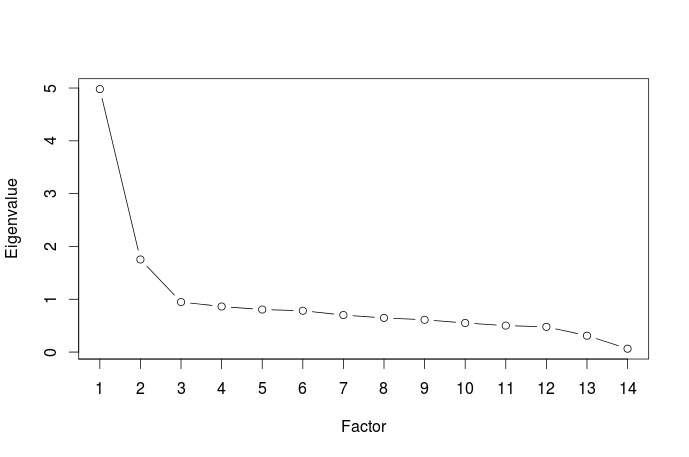
\includegraphics[width=0.8\linewidth]{pca-eigenvalues.png}
  \caption{Scree test: eigenvalues by factor}
  \label{fig:pca-eigenvalues}
\end{figure}

Figure~\ref{fig:pca-eigenvalues} shows scree test elbow occurs around 2 or 3. Also, eigenvalues 1 and $2 > 1$, while 3
is around .9

\section{$k$-means}
\subsection{Identifying optimal number of clusters}

\subsubsection{WSS Error Scree Test}

\begin{figure}[ht]
  \centering
  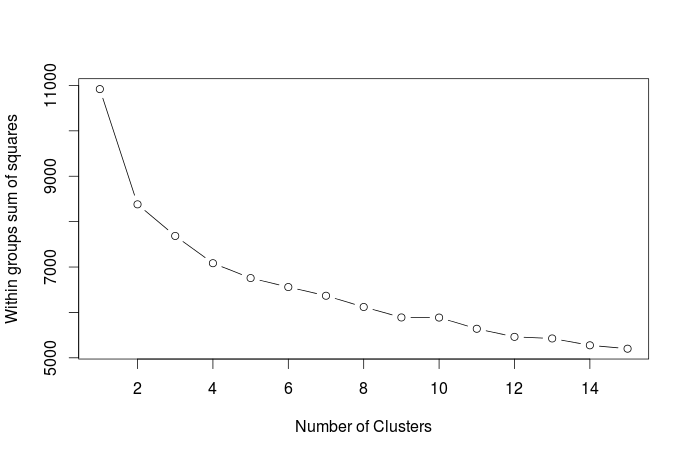
\includegraphics[width=0.8\linewidth]{kmeans-wss-error.png}
  \caption{Scree test: WSS error by cluster size}
  \label{fig:kmeans-wss-error}
\end{figure}

Figure~\ref{fig:kmeans-wss-error} shows no optimal elbow in scree test! Maybe 2-3?

\subsubsection{Gap Statistic}

Optimal cluster is the local maximum of the gap statistic, but it appears to be
consistently increasing in Figure~\ref{fig:gap-statistic}.

\begin{figure}[ht]
  \centering
  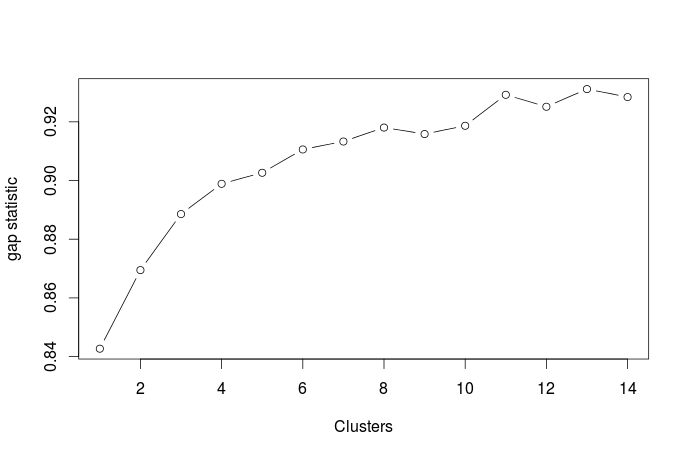
\includegraphics[width=0.8\linewidth]{gap-statistic.png}
  \caption{Gap statistic by cluster size}
  \label{fig:gap-statistic}
\end{figure}

\subsubsection{Average Silhouette Width}

Figure~\ref{fig:asw} shows average silhouette width as being consistently under
0.25 for all clusters, implying the data is not well structured.

\begin{figure}[ht]
  \centering
  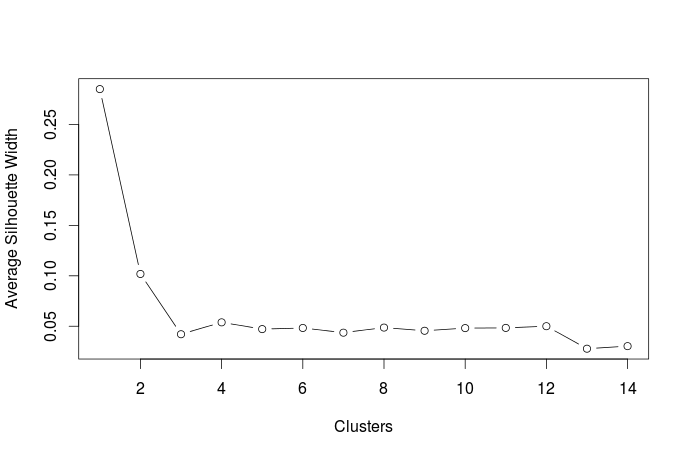
\includegraphics[width=0.8\linewidth]{asw.png}
  \caption{Average silhouette width by cluster size}
  \label{fig:asw}
\end{figure}

% \subsubsection{\texttt{NbClust} package}

\subsection{Cluster statistics}
% CLUSTERS: 2
% ================================
% Sizes: 201 580
% WithinSS: 4248.585 4132.434
% Sum WithinSS: 8381.019
% CLUSTERS: 3
% ================================
% Sizes: 420 231 130
% WithinSS: 2618.368 1973.82 3076.542
% Sum WithinSS: 7668.73
% CLUSTERS: 4
% ================================
% Sizes: 61 372 145 203
% WithinSS: 1481.25 1845.389 2147.988 1609.555
% Sum WithinSS: 7084.183
\begin{table}[ht]
  \centering
  \begin{tabular}{l|l|l|l}
    $k$ & $n$ & Within SS & sum(Within SS) \\
    \hline
    2 & 201/580 & 4248.585/4132.434 & 8381.019 \\
    3 & 420/231/130 & 2618.368/1973.82/3076.542 &  7668.73 \\
    4 & 61/372/145/203 & 1481.25/1845.389/2147.988/1609.555 & 7084.183
  \end{tabular}
  \caption{Cluster statistics}
  \label{tab:cluster-statistics}
\end{table}

\subsection{Centers}
Omitted; too much information.
\iffalse
\begin{lstlisting}
CLUSTERS: 2
================================
> 1   nms_d1    nms_d2    nms_d3    nms_d4    nms_d5    nms_d6    nms_d7    nms_d8    nms_d9    tremor  bradykin
0.7328282 0.9345720 0.9810287 0.8195052 0.7908599 0.8551764 0.8493069 0.6376458 0.6289463 0.2008254 0.8019272
 rigidity     axial      pigd
0.6840038 1.0834910 1.0634082
> 2    nms_d1     nms_d2     nms_d3     nms_d4     nms_d5     nms_d6     nms_d7     nms_d8     nms_d9     tremor
-0.2539629 -0.3238776 -0.3399772 -0.2840009 -0.2740739 -0.2963629 -0.2943288 -0.2209772 -0.2179624 -0.0695964
  bradykin   rigidity      axial       pigd
-0.2779093 -0.2370427 -0.3754857 -0.3685259
CLUSTERS: 3
================================
> 1    nms_d1     nms_d2     nms_d3     nms_d4     nms_d5     nms_d6     nms_d7     nms_d8     nms_d9     tremor
-0.2699345 -0.3571672 -0.3574942 -0.2776501 -0.2579928 -0.3084614 -0.3030016 -0.2270260 -0.1867338 -0.2531402
  bradykin   rigidity      axial       pigd
-0.6091393 -0.5542033 -0.5792769 -0.5775312
> 2     nms_d1      nms_d2      nms_d3      nms_d4      nms_d5      nms_d6      nms_d7      nms_d8      nms_d9
-0.13369057 -0.07938936 -0.05832302 -0.22742096 -0.18981647 -0.02540265 -0.15964421 -0.08973885 -0.16993231
     tremor    bradykin    rigidity       axial        pigd
 0.39256552  0.69210577  0.63956741  0.43974428  0.44762184
> 3   nms_d1    nms_d2    nms_d3    nms_d4    nms_d5    nms_d6    nms_d7    nms_d8    nms_d9    tremor  bradykin
1.1096539 1.2949935 1.2586166 1.3011330 1.1708044 1.0417061 1.2626038 0.8929277 0.9052504 0.1202787 0.7381697
 rigidity     axial      pigd
0.6540408 1.0901181 1.0704805
CLUSTERS: 4
================================
> 1   nms_d1    nms_d2    nms_d3    nms_d4    nms_d5    nms_d6    nms_d7    nms_d8    nms_d9    tremor  bradykin
1.5558981 1.4133002 1.1184738 1.9877193 1.2550406 1.5834288 1.4194860 0.7793719 0.8480830 0.4984324 1.5155436
 rigidity     axial      pigd
1.5055810 1.9495563 1.9242566
> 2    nms_d1     nms_d2     nms_d3     nms_d4     nms_d5     nms_d6     nms_d7     nms_d8     nms_d9     tremor
-0.3206187 -0.4993585 -0.4670797 -0.3084269 -0.3380326 -0.3885648 -0.3868053 -0.2817080 -0.3620072 -0.2526726
  bradykin   rigidity      axial       pigd
-0.5841212 -0.5460419 -0.5968519 -0.5927227
> 3     nms_d1      nms_d2      nms_d3      nms_d4      nms_d5      nms_d6      nms_d7      nms_d8      nms_d9
 0.35964469  0.82182933  0.92114183  0.30981044  0.75178256  0.42320932  0.66431905  0.63701383  0.85893238
     tremor    bradykin    rigidity       axial        pigd
-0.34050774 -0.15173201 -0.20269121  0.04852427  0.04032785
> 4     nms_d1      nms_d2      nms_d3      nms_d4      nms_d5      nms_d6      nms_d7      nms_d8      nms_d9
-0.13688715 -0.09662665 -0.13812235 -0.25339210 -0.29466914 -0.06605132 -0.19223309 -0.17297198 -0.20498319
     tremor    bradykin    rigidity       axial        pigd
 0.55647025  0.72337965  0.69299204  0.47325105  0.47914113
\end{lstlisting}
\fi

\subsection{Decision tree classifier based on clusters}
% seed = 911
% CLUSTERS: 2
% ================================
% Complexity Parameter: 0.03482587
% 10-fold CV error: 0.134443
% Root node error: 0.2573624
% CLUSTERS: 3
% ================================
% Complexity Parameter: 0.01
% 10-fold CV error: 0.1946223
% Root node error: 0.4622279
% CLUSTERS: 4
% ================================
% Complexity Parameter: 0.01
% 10-fold CV error: 0.2483995
% Root node error: 0.5236876
\begin{table}[ht]
  \centering
  \begin{tabular}{l|l|l|l|l|l}
    $k$ & CP\tablefootnote{Complexity Parameter} & CV Xerror\tablefootnote{10-fold cross
    validation} & Root Feature &
    Root Error & Figure \\
    \hline
    2 & 0.0348 & 0.134 & axial $\geq$ 0.44 & 0.257 & Figure~\ref{fig:kmeans-dtree-2} \\
    3 & 0.0100 & 0.194 & bradykin $<$ 0.0041 & 0.462 & Figure~\ref{fig:kmeans-dtree-3} \\
    4 & 0.0100 & 0.248 & bradykin $<$ 0.0041 & 0.523 & Figure~\ref{fig:kmeans-dtree-4} \\
  \end{tabular}
  \caption{$k$-kmeans decision trees statistics}
  \label{tab:k-means-dtrees}
\end{table}

\begin{figure}[ht]
  \centering
  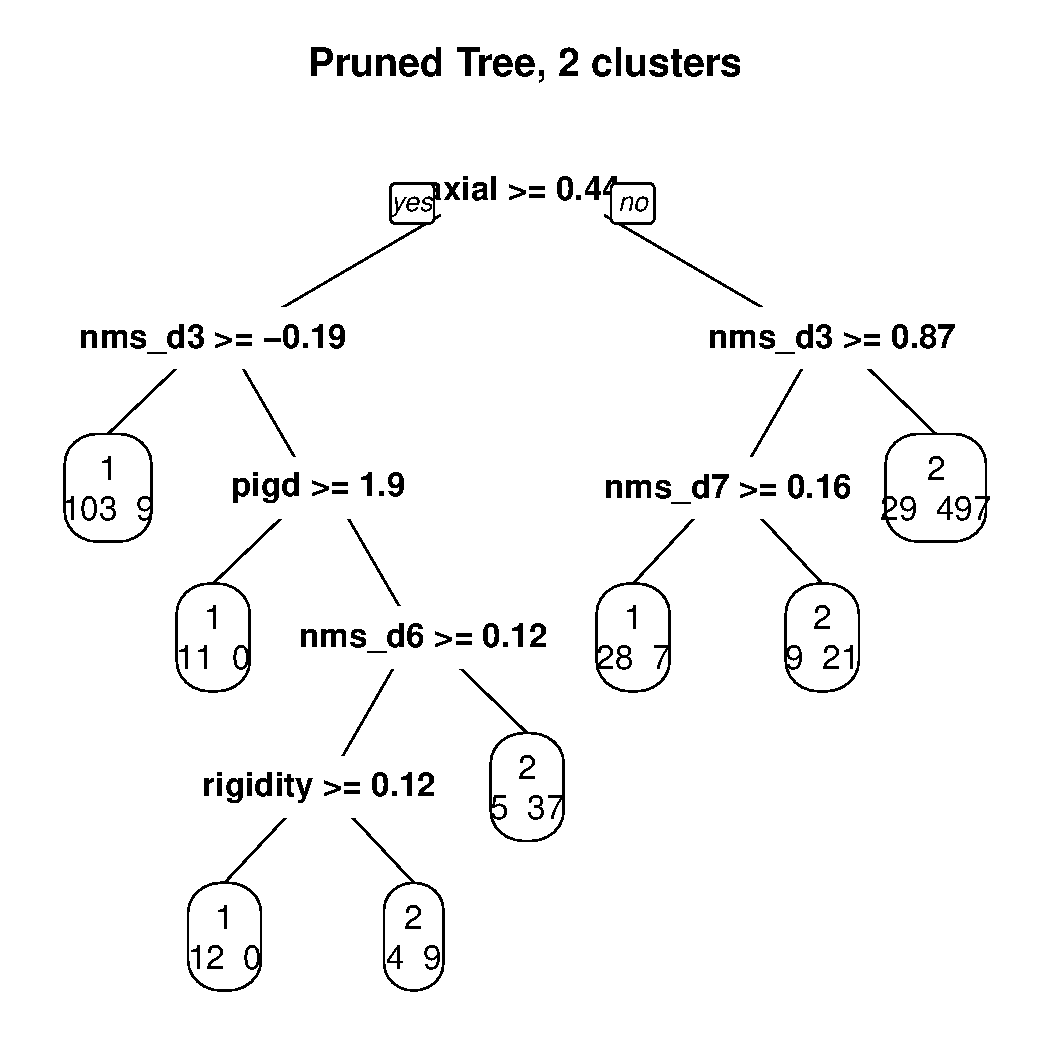
\includegraphics[width=0.8\linewidth]{dtree-kmeans-pruned-2.pdf}
  \caption{Decision Tree from $k$-means clustering, 2 clusters}
  \label{fig:kmeans-dtree-2}
\end{figure}

\begin{figure}[ht]
  \centering
  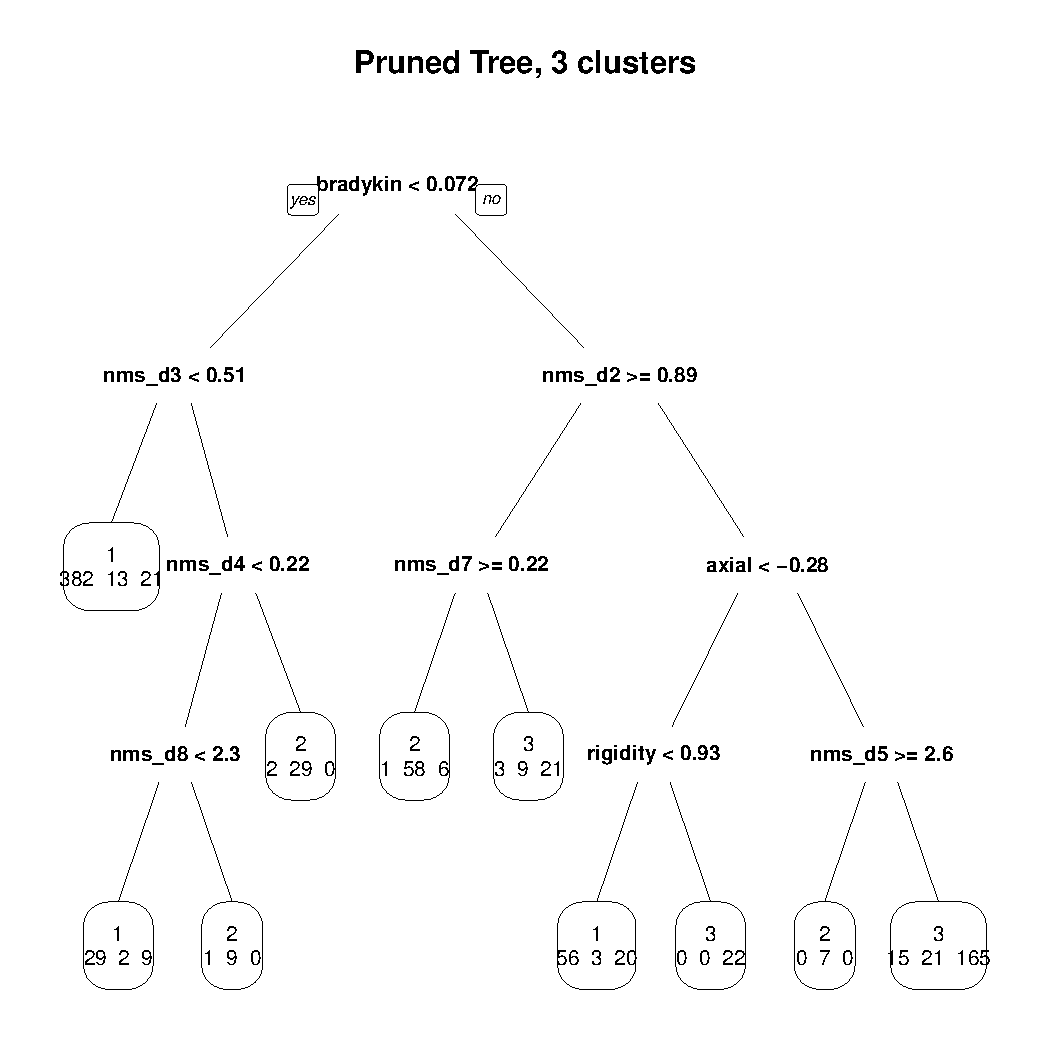
\includegraphics[width=0.8\linewidth]{dtree-kmeans-pruned-3.pdf}
  \caption{Decision Tree from $k$-means clustering, 3 clusters}
  \label{fig:kmeans-dtree-3}
\end{figure}

\begin{figure}[ht]
  \centering
  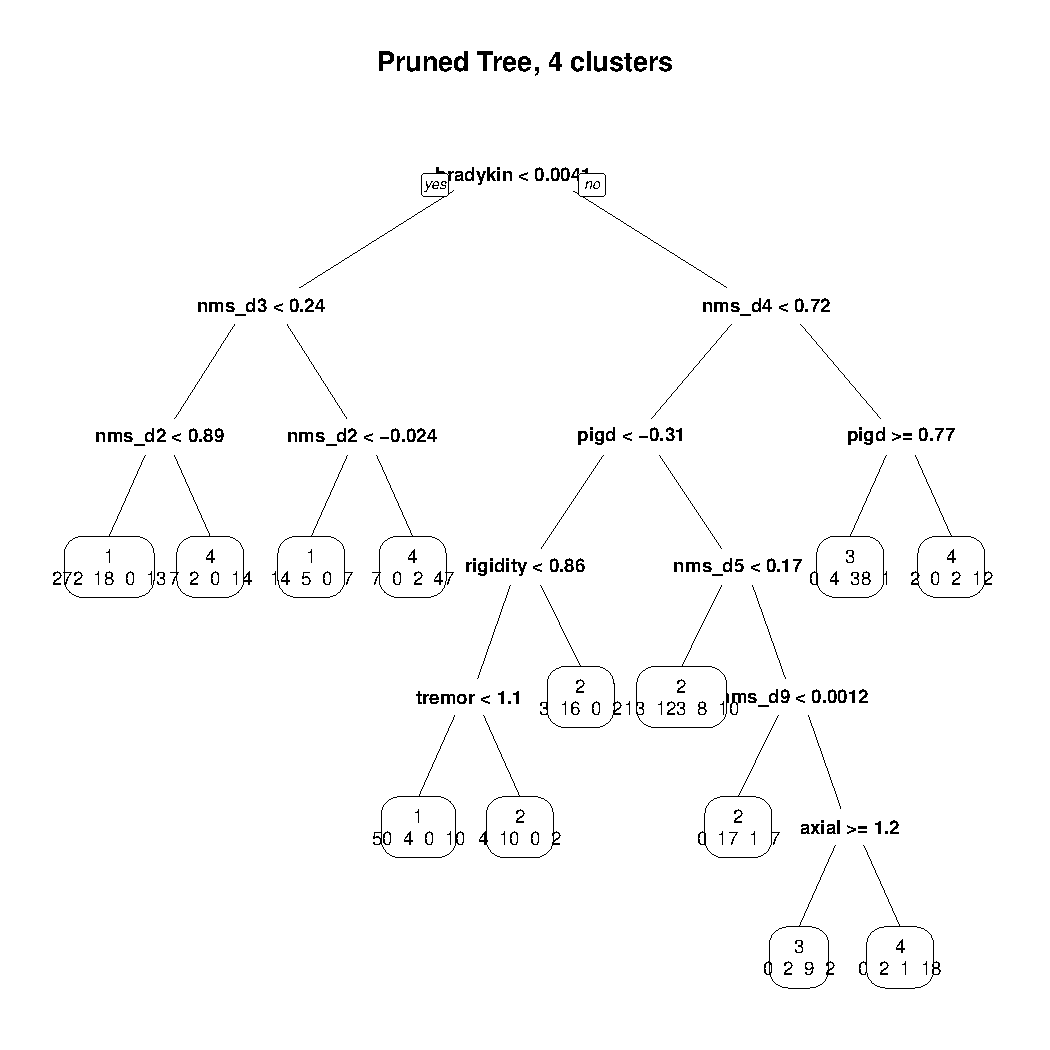
\includegraphics[width=0.8\linewidth]{dtree-kmeans-pruned-4.pdf}
  \caption{Decision Tree from $k$-means clustering, 4 clusters}
  \label{fig:kmeans-dtree-4}
\end{figure}

\subsection{Summary Statistics based on Clusters}

\begin{lstlisting}
k = 2, cluster 1
var,mean,sd,min,max
age,68.38,9.4,42,89
sex,0.43,0.5,0,1
pdonset,57.65,10.81,32,87
durat_pd,10.73,7.14,0,40
cisitot,13.07,4.55,2,24
k = 2, cluster 2
var,mean,sd,min,max
age,63.43,9.55,37,89
sex,0.36,0.48,0,1
pdonset,56.44,10.62,28,89
durat_pd,6.99,4.94,0,28
cisitot,6.64,3.42,0,16

k = 3, cluster 1
var,mean,sd,min,max
age,62.69,9.43,37,89
sex,0.39,0.49,0,1
pdonset,56.04,10.41,28,89
durat_pd,6.65,4.66,0,26
cisitot,5.76,3.15,0,15
k = 3, cluster 2
var,mean,sd,min,max
age,66.17,9.74,38,86
sex,0.32,0.47,0,1
pdonset,57.78,11.19,32,84
durat_pd,8.39,5.79,0,31
cisitot,9.95,3.5,2,22
k = 3, cluster 3
var,mean,sd,min,max
age,68.62,9.2,50,89
sex,0.46,0.5,0,1
pdonset,57.24,10.46,35,87
durat_pd,11.38,7.52,0,40
cisitot,13.52,5.01,2,24

k = 4, cluster 1
var,mean,sd,min,max
age,71.9,8.1,54,89
sex,0.46,0.5,0,1
pdonset,58.28,10.27,35,87
durat_pd,13.62,7.76,0,40
cisitot,16.72,4.14,4,24
k = 4, cluster 2
var,mean,sd,min,max
age,62.65,9.63,37,89
sex,0.36,0.48,0,1
pdonset,56.13,10.47,28,89
durat_pd,6.52,4.66,0,25
cisitot,5.58,3.12,0,15
k = 4, cluster 3
var,mean,sd,min,max
age,64.79,9.3,44,86
sex,0.47,0.5,0,1
pdonset,56.2,10.71,35,85
durat_pd,8.59,6.16,0,27
cisitot,9.23,3.88,2,19
k = 4, cluster 4
var,mean,sd,min,max
age,66.27,9.47,40,86
sex,0.33,0.47,0,1
pdonset,57.84,11.06,32,84
durat_pd,8.43,5.64,0,31
cisitot,10.06,3.49,3,22
\end{lstlisting}
\section{Biclustering}

Used BCBimax clustering algorithm. Clusters seem quite sparse.

\begin{figure}[ht]
  \centering
  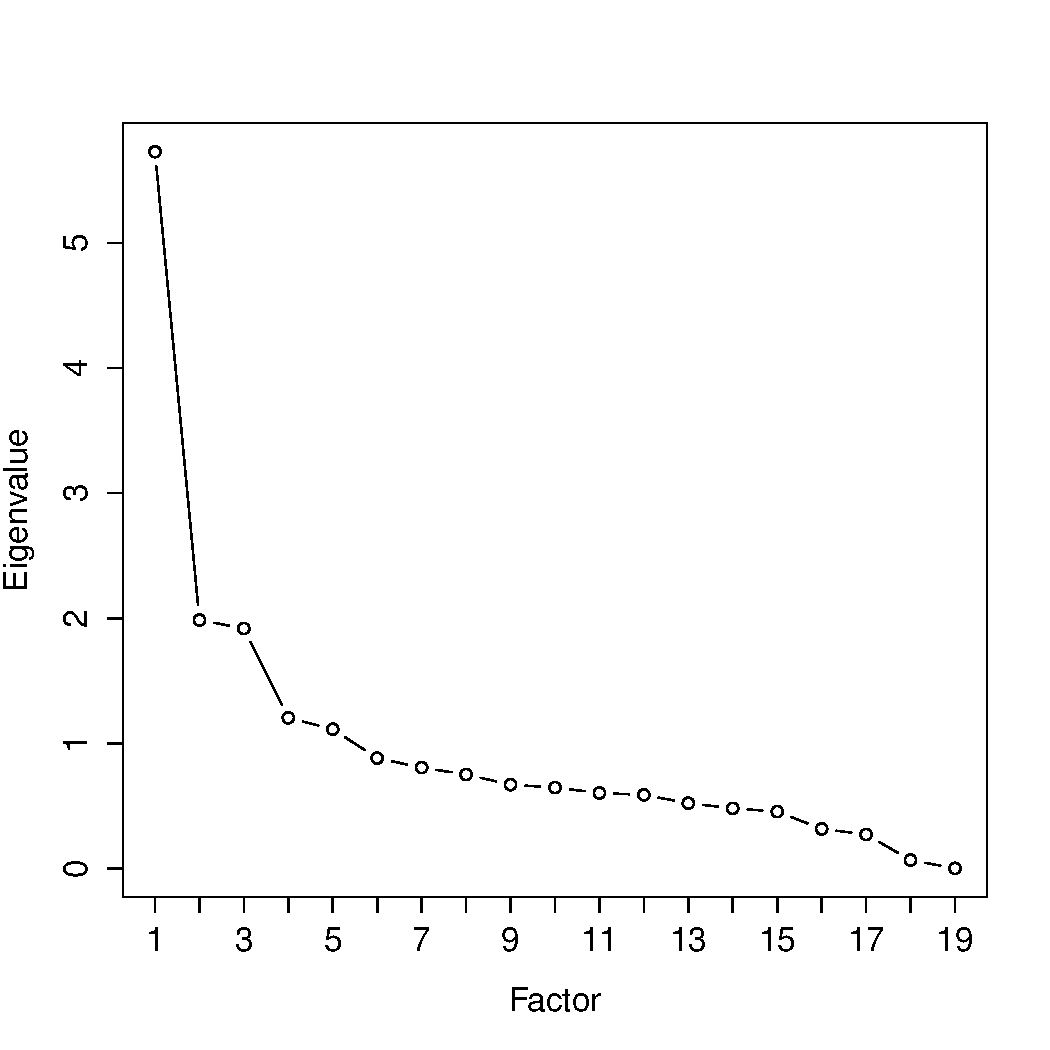
\includegraphics[width=0.8\linewidth]{biclust-16.pdf}
  \caption{Biclustering $N = 16$}
  \label{fig:biclust-16}
\end{figure}

\begin{figure}[ht]
  \centering
  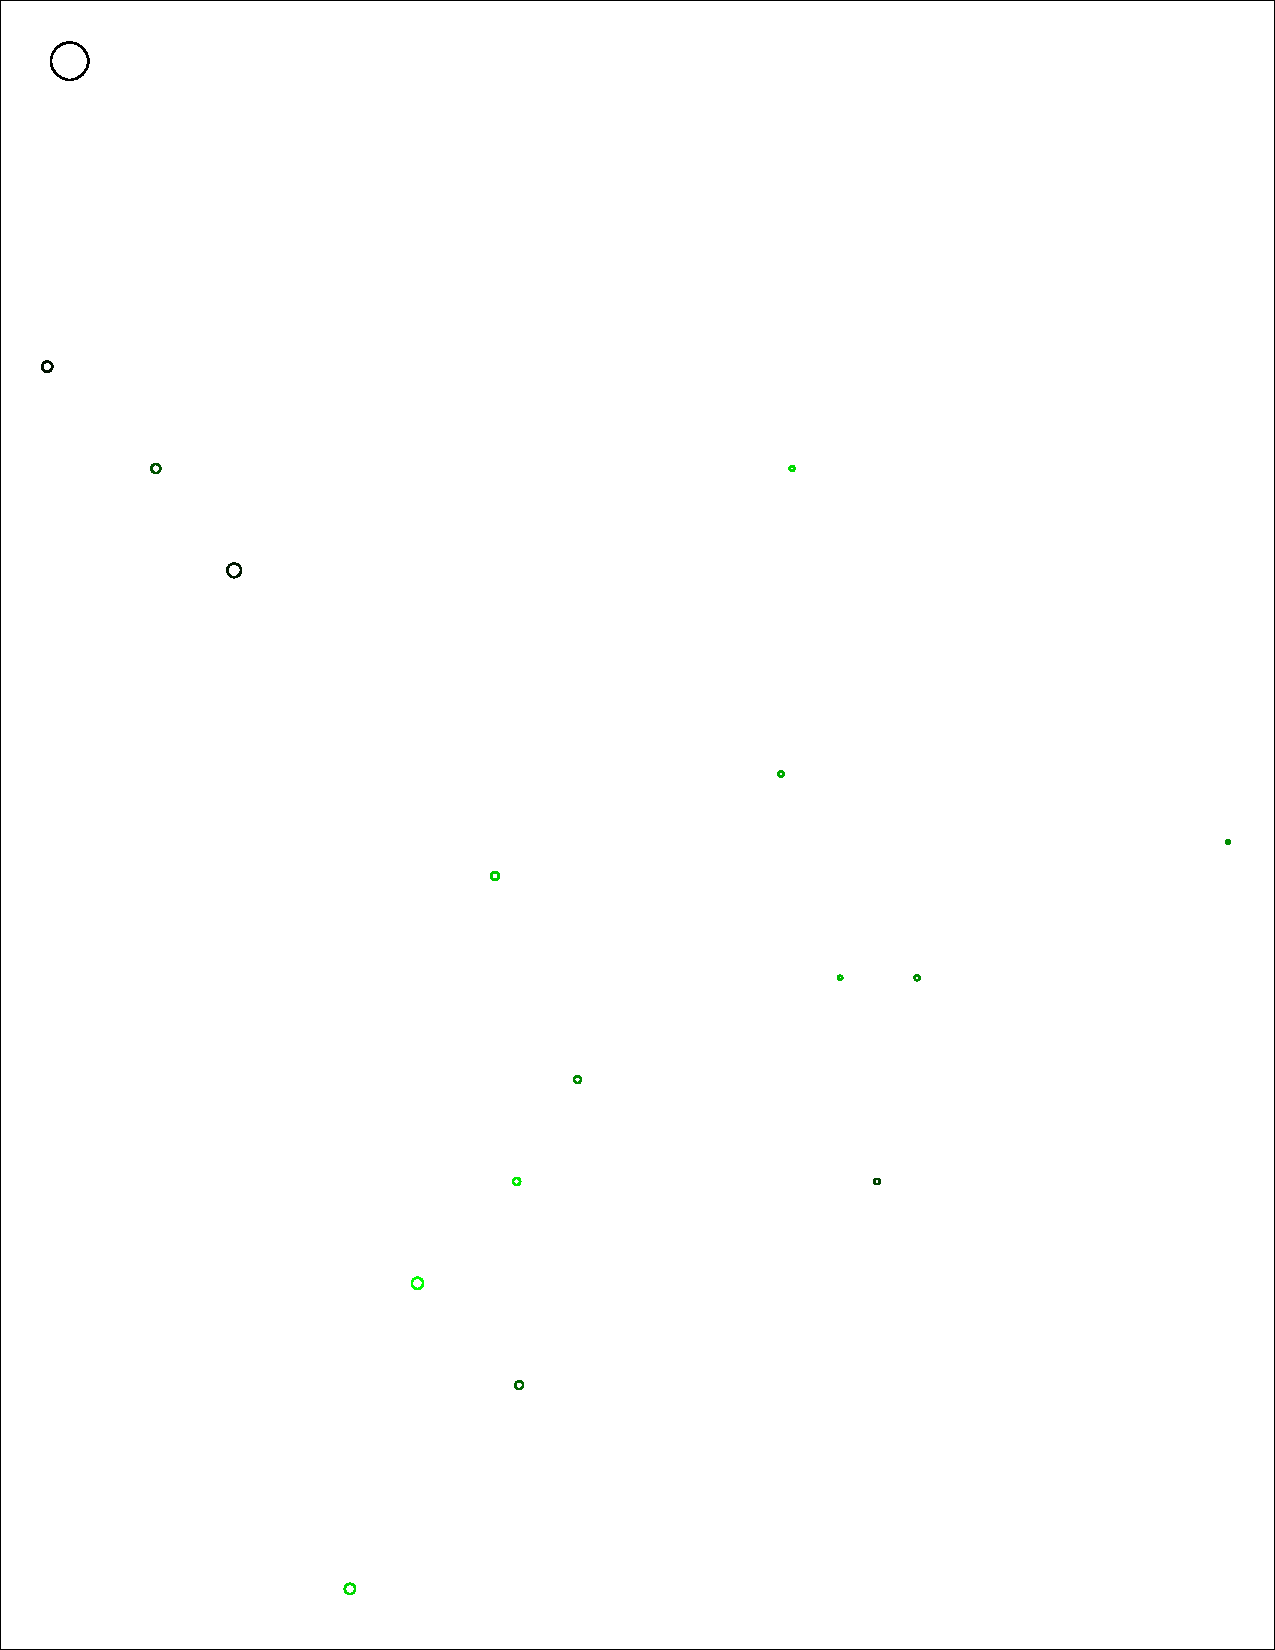
\includegraphics[width=0.8\linewidth]{bubbleplot-16.pdf}
  \caption{Bubbleplot $N = 16$}
  \label{fig:bubbleplot-16}
\end{figure}

\section{Subspace clustering}

% TODO: Wat.

\section{Bayesian Networks}

\end{document}
